% ==========================================================
% WEEK 2 — MODELS OF DISTRIBUTED COMPUTATION
% CHUNK A — SLIDES 1–10
% PROBLEM → DIAGRAM → SOLUTION (separate slides)
% ==========================================================

% ----------------------------------------------------------
\section{Framing the Discipline}
% ----------------------------------------------------------

\begin{frame}{Distributed Computation is Hard}
\begin{block}{Problem}
Distributed systems consist of independently executing processes that communicate over unreliable networks. Each process has only a partial, delayed, and inconsistent view of global state.
\end{block}

\begin{center}
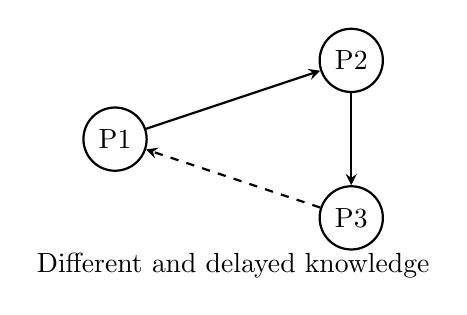
\begin{tikzpicture}[>=stealth, thick]
\node[draw,circle] (p1) at (0,0){P1};
\node[draw,circle] (p2) at (3,1){P2};
\node[draw,circle] (p3) at (3,-1){P3};

\draw[->] (p1) -- (p2);
\draw[->] (p2) -- (p3);
\draw[->,dashed] (p3) -- (p1);

\node at (1.5,-1.6){Different and delayed knowledge};
\end{tikzpicture}
\end{center}
\end{frame}

\begin{frame}{Distributed Computation — Solutions}
\begin{itemize}
    \item \textbf{Logical clocks} for ordering without synchronized time.
    \item \textbf{Quorum-based decisions} instead of global agreement.
    \item \textbf{Replicated state machines} for deterministic consistency.
    \item \textbf{Retry and reconciliation} to overcome uncertainty.
    \item \textbf{Failure detectors} to approximate liveness information.
\end{itemize}
\end{frame}

% ----------------------------------------------------------
\section{Asynchrony}
% ----------------------------------------------------------

\begin{frame}{Asynchrony}
\begin{block}{Problem}
Message delays are unbounded. A node cannot distinguish a slow peer from a failed or partitioned one. Silence has no meaning.
\end{block}

\begin{center}
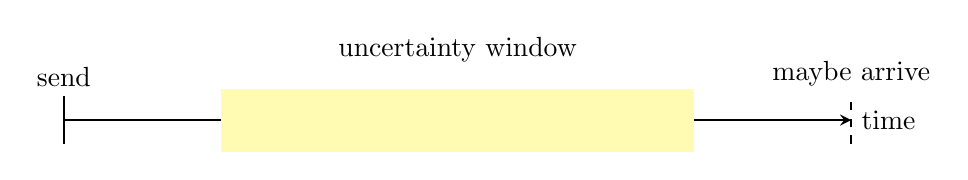
\begin{tikzpicture}[>=stealth, thick]
\draw[->] (0,0)--(10,0) node[right]{time};

\fill[yellow!30] (2,-0.4) rectangle (8,0.4);
\node at (5,0.9){uncertainty window};

\draw (0,-0.3)--(0,0.3) node[above]{send};
\draw[dashed] (10,-0.3)--(10,0.3) node[above]{maybe arrive};
\end{tikzpicture}
\end{center}
\end{frame}

\begin{frame}{Asynchrony — Solutions}
\begin{itemize}
    \item \textbf{Partial synchrony assumptions} for eventual timing bounds.
    \item \textbf{Randomized timeouts} to avoid synchronized failure.
    \item \textbf{Quorum reads/writes} to avoid waiting for all nodes.
    \item \textbf{Eventual failure detectors} that improve over time.
    \item \textbf{Logical ordering} instead of timing-based decisions.
\end{itemize}
\end{frame}

% -----------------------------------------------------------
\section{Timeout Ambiguity}
% -----------------------------------------------------------

\begin{frame}{Timeout Ambiguity}
\begin{block}{Problem}
A timeout indicates missing messages, not a crash. Reacting prematurely can cause split-brain or two leaders if delayed messages later arrive.
\end{block}

\begin{center}
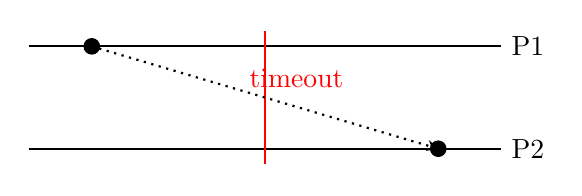
\begin{tikzpicture}[>=stealth, thick]

\draw (0,0) -- (6,0) node[right]{P1};
\draw (0,-1.3) -- (6,-1.3) node[right]{P2};

\fill (0.8,0) circle(3pt);
\draw[red,thick] (3,0.2)--(3,-1.5);
\node[red] at (3.4,-0.4){timeout};

\fill (5.2,-1.3) circle(3pt);
\draw[->,dotted] (0.8,0)--(5.2,-1.3);

\end{tikzpicture}
\end{center}
\end{frame}

\begin{frame}{Timeout Ambiguity — Solutions}
\begin{itemize}
    \item \textbf{Terms/epochs} invalidate outdated leaders (Raft).
    \item \textbf{Leases} provide time-bounded authority.
    \item \textbf{Commit rules} require quorum confirmation.
    \item \textbf{Redundant communication} to detect restored nodes.
    \item \textbf{Delayed leadership transition} to avoid flapping.
\end{itemize}
\end{frame}

% ----------------------------------------------------------
\section{Timing Models}
% ----------------------------------------------------------

\begin{frame}{Synchronous Model}
\begin{block}{Problem}
The synchronous model assumes predictable message and processing times. Real systems rarely meet these assumptions, causing synchronous algorithms to fail under modest delay.
\end{block}

\begin{center}
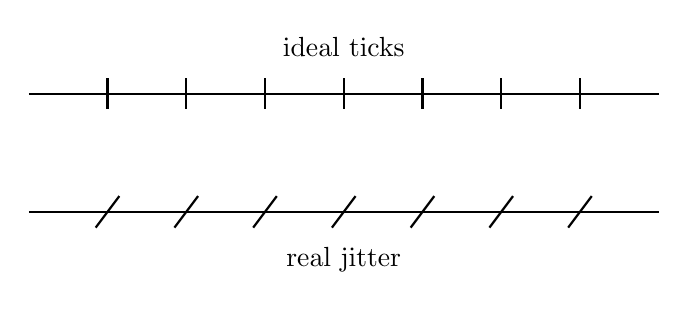
\begin{tikzpicture}[>=stealth, thick]
\draw (0,0)--(8,0);
\foreach \t in {1,...,7}{\draw (\t,0.2)--(\t,-0.2);}
\node at (4,0.6){ideal ticks};

\draw (0,-1.5)--(8,-1.5);
\foreach \t in {1,...,7}{\draw (\t+0.15,-1.3)--(\t-0.15,-1.7);}
\node at (4,-2.1){real jitter};
\end{tikzpicture}
\end{center}
\end{frame}

\begin{frame}{Synchronous Model — Solutions}
\begin{itemize}
    \item \textbf{Treat synchrony as conceptual only}.
    \item \textbf{Design protocols for weaker models} (e.g., Raft, Paxos).
    \item \textbf{Avoid timing-based correctness assumptions}.
    \item \textbf{Use timeouts as hints, not proofs of failure}.
    \item \textbf{Use logical clocks} when real time is unreliable.
\end{itemize}
\end{frame}

% ==========================================================
% WEEK 2 — MODELS OF DISTRIBUTED COMPUTATION
% CHUNK B — SLIDES 11–20
% PROBLEM → DIAGRAM → SOLUTION
% ==========================================================

% ----------------------------------------------------------
\section{Communication Uncertainty}
% ----------------------------------------------------------

% ---------- Slide 11 ----------
\begin{frame}{Message Reordering}
\begin{block}{Problem}
Messages may traverse different network paths or face variable queueing delays. As a result, they can arrive in an order different from the one in which they were sent.
\end{block}

\begin{center}
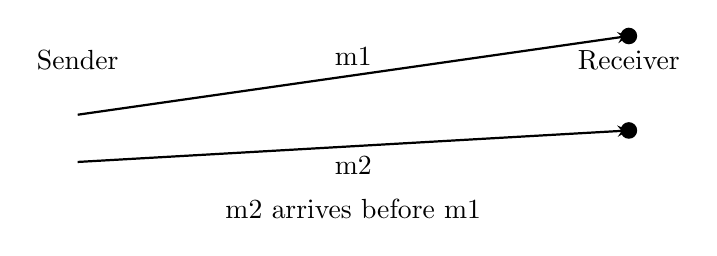
\begin{tikzpicture}[>=stealth, thick]
\node at (0,0.7){Sender};
\node at (7,0.7){Receiver};

\draw[->] (0,0) -- (7,1.0) node[midway,above]{m1};
\draw[->] (0,-0.6) -- (7,-0.2) node[midway,below]{m2};

\fill (7,1.0) circle(3pt);
\fill (7,-0.2) circle(3pt);

\node at (3.5,-1.2){m2 arrives before m1};
\end{tikzpicture}
\end{center}
\end{frame}

% ---------- Slide 12 ----------
\begin{frame}{Message Reordering — Solutions}
\begin{itemize}
    \item \textbf{Sequence numbers} to restore intended order.
    \item \textbf{Version vectors} to track causality across replicas.
    \item \textbf{Idempotent operations} to tolerate duplicates.
    \item \textbf{Deterministic replay} in replicated state machines.
    \item \textbf{Ordering layers} such as TCP or application-level queues.
\end{itemize}
\end{frame}

% ---------- Slide 13 ----------
\begin{frame}{Message Loss}
\begin{block}{Problem}
Networks drop messages due to congestion, queue overflow, or transient link faults. Loss prevents updates from propagating and may leave replicas inconsistent.
\end{block}

\begin{center}
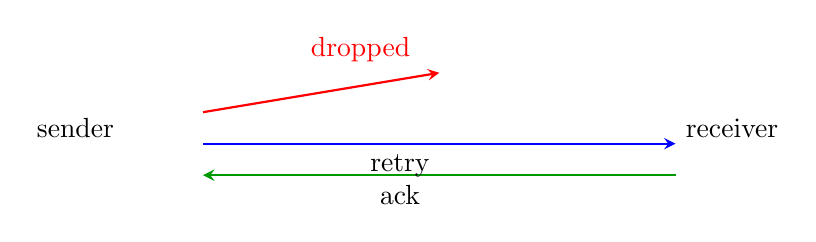
\begin{tikzpicture}[>=stealth, thick]
\node[left] at (0,0){sender};
\node[right] at (7,0){receiver};

\draw[->,red] (1,0.2) -- (4,0.7);
\node[red] at (3,1.0){dropped};

\draw[->,blue] (1,-0.2) -- (7,-0.2);
\draw[->,green!60!black] (7,-0.6) -- (1,-0.6);

\node[below] at (3.5,-0.2){retry};
\node[below] at (3.5,-0.6){ack};
\end{tikzpicture}
\end{center}
\end{frame}

% ---------- Slide 14 ----------
\begin{frame}{Message Loss — Solutions}
\begin{itemize}
    \item \textbf{Retransmissions} until confirmation is received.
    \item \textbf{Acknowledgments} to confirm delivery.
    \item \textbf{Checksums} to detect corruption.
    \item \textbf{Backoff algorithms} to reduce congestion.
    \item \textbf{Periodic anti-entropy} to reconcile state.
\end{itemize}
\end{frame}

% ---------- Slide 15 ----------
\begin{frame}{Arbitrary Delay}
\begin{block}{Problem}
Messages may be delayed indefinitely. Such delays look identical to failures, making timing unreliable for determining remote state or coordinating decisions.
\end{block}

\begin{center}
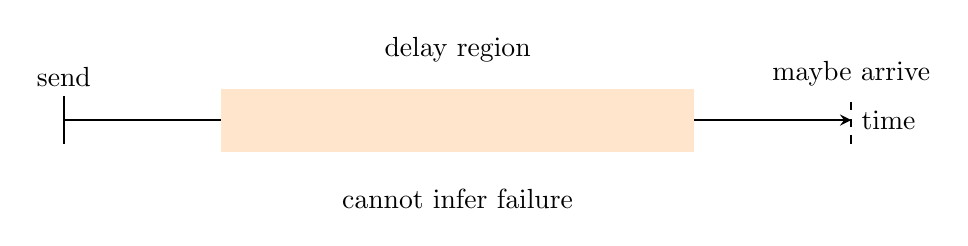
\begin{tikzpicture}[>=stealth, thick]
\draw[->] (0,0) -- (10,0) node[right]{time};

\fill[orange!20] (2,-0.4) rectangle (8,0.4);
\node at (5,0.9){delay region};

\draw (0,-0.3)--(0,0.3) node[above]{send};
\draw[dashed] (10,-0.3)--(10,0.3) node[above]{maybe arrive};

\node at (5,-1.0){cannot infer failure};
\end{tikzpicture}
\end{center}
\end{frame}

% ---------- Slide 16 ----------
\begin{frame}{Arbitrary Delay — Solutions}
\begin{itemize}
    \item \textbf{Quorum-based operations} to tolerate missing responses.
    \item \textbf{Randomized timeouts} to reduce coordination conflicts.
    \item \textbf{Eventually perfect failure detectors} improving over time.
    \item \textbf{Epoch-based leadership} to avoid split-brain.
    \item \textbf{Delay-independent safety rules} in consensus protocols.
\end{itemize}
\end{frame}

% ----------------------------------------------------------
\section{Correctness Under Uncertainty}
% ----------------------------------------------------------

% ---------- Slide 17 ----------
\begin{frame}{Safety}
\begin{block}{Problem}
A system violates safety if it reaches an invalid state—such as electing two leaders or committing conflicting operations. Safety violations cannot be undone once they occur.
\end{block}

\begin{center}
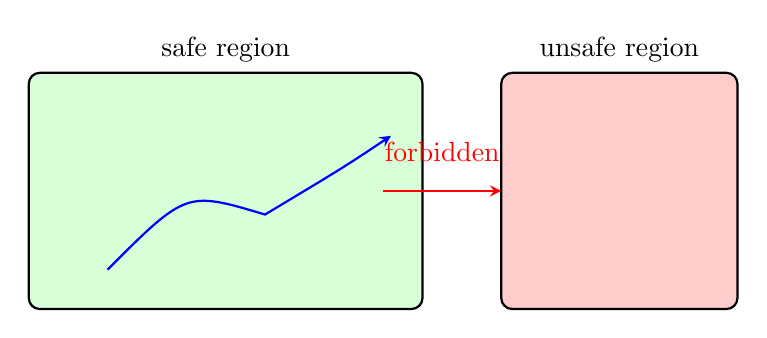
\begin{tikzpicture}[>=stealth, thick]

\draw[fill=green!15,rounded corners] (0,0) rectangle (5,3);
\node at (2.5,3.3){safe region};

\draw[fill=red!20,rounded corners] (6,0) rectangle (9,3);
\node at (7.5,3.3){unsafe region};

\draw[blue,thick,->]
  (1,0.5) .. controls (2,1.5) .. (3,1.2)
          .. controls (4,1.8) .. (4.6,2.2);

\draw[red,thick,->] (4.5,1.5) -- (6,1.5);
\node[red] at (5.25,2.0){forbidden};
\end{tikzpicture}
\end{center}
\end{frame}

% ---------- Slide 18 ----------
\begin{frame}{Safety — Solutions}
\begin{itemize}
    \item \textbf{Single-writer leadership} to serialize decisions.
    \item \textbf{State machine replication} for deterministic behavior.
    \item \textbf{Quorum-based commits} to avoid conflicting decisions.
    \item \textbf{Monotonic state transitions} (legal state space).
    \item \textbf{Invariant-preserving protocols} such as Raft/Paxos.
\end{itemize}
\end{frame}

% ---------- Slide 19 ----------
\begin{frame}{Liveness}
\begin{block}{Problem}
Even if safety holds, a system may stall indefinitely under heavy delay or unstable leadership. Liveness requires eventual forward progress.
\end{block}

\begin{center}
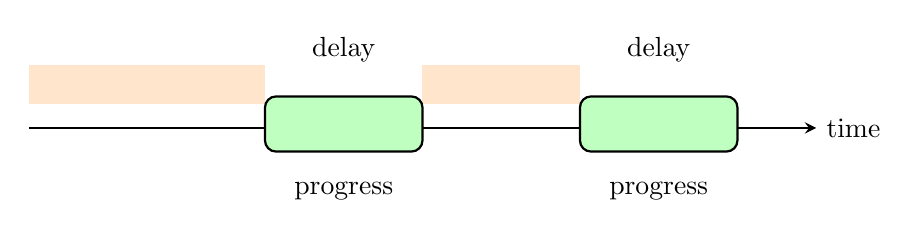
\begin{tikzpicture}[>=stealth, thick]
\draw[->] (0,0) -- (10,0) node[right]{time};

\fill[orange!20] (0,0.3) rectangle (3,0.8);
\fill[orange!20] (5,0.3) rectangle (7,0.8);

\draw[fill=green!25,rounded corners] (3,-0.3) rectangle (5,0.4);
\draw[fill=green!25,rounded corners] (7,-0.3) rectangle (9,0.4);

\node at (4,1.0){delay};
\node at (8,1.0){delay};
\node at (4,-0.8){progress};
\node at (8,-0.8){progress};
\end{tikzpicture}
\end{center}
\end{frame}

% ---------- Slide 20 ----------
\begin{frame}{Liveness — Solutions}
\begin{itemize}
    \item \textbf{Randomized leader election} to break symmetry.
    \item \textbf{Eventually stable timeouts} after network recovery.
    \item \textbf{Retry loops} to ensure completion under partial failure.
    \item \textbf{Failure detectors} that improve accuracy over time.
    \item \textbf{Progress conditions} built into consensus protocols.
\end{itemize}
\end{frame}

\begin{algorithm}[H]
\footnotesize
\caption{Retry-with-Ack Protocol}
\begin{algorithmic}[1]
\State send(msg)
\While{no ack received}
    \State wait(timeout)
    \State resend(msg)
\EndWhile
\end{algorithmic}
\end{algorithm}

% ==========================================================
% WEEK 2 — MODELS OF DISTRIBUTED COMPUTATION
% CHUNK C — SLIDES 21–30
% PROBLEM → DIAGRAM → SOLUTION (+ alternating algorithms)
% ==========================================================

% ----------------------------------------------------------
\section{Eventual Consistency and CRDTs}
% ----------------------------------------------------------

% ---------- Slide 21 ----------
\begin{frame}{Eventual Consistency}
\begin{block}{Problem}
Replicas receive updates in different orders and at different times. Without coordination, their states may temporarily diverge, producing inconsistent reads across the system.
\end{block}

\begin{center}
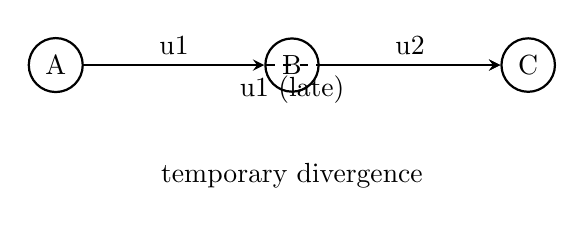
\begin{tikzpicture}[>=stealth, thick]
\node[draw,circle] (a) at (0,1){A};
\node[draw,circle] (b) at (3,1){B};
\node[draw,circle] (c) at (6,1){C};

\draw[->] (a) -- (b) node[midway,above]{u1};
\draw[->,dashed] (a) -- (c) node[midway,below]{u1 (late)};
\draw[->] (b) -- (c) node[midway,above]{u2};

\node at (3,-0.4){temporary divergence};
\end{tikzpicture}
\end{center}
\end{frame}

% ---------- Slide 22 ----------
\begin{frame}{Eventual Consistency — Solutions}
\begin{itemize}
    \item \textbf{Anti-entropy protocols} to exchange and reconcile state.
    \item \textbf{Version vectors} for detecting missing causal updates.
    \item \textbf{Idempotent updates} to tolerate replay and duplicates.
    \item \textbf{Convergent conflict-resolution rules} (e.g., LWW).
    \item \textbf{Periodic gossip} for reliable dissemination.
\end{itemize}
\end{frame}

% ---------- Slide 23 ----------
\begin{frame}{Eventual Consistency — Anti-Entropy Algorithm}
\begin{algorithm}[H]
\footnotesize
\caption{Periodic Anti-Entropy}
\begin{algorithmic}[1]
\While{true}
    \State wait(random\_interval())
    \State peer $\gets$ pickRandomReplica()
    \State send(localState, peer)
    \State remoteState $\gets$ receive(peer)
    \State localState $\gets$ merge(localState, remoteState)
\EndWhile
\end{algorithmic}
\end{algorithm}
\end{frame}

% ----------------------------------------------------------
\section{CRDTs}
% ----------------------------------------------------------

% ---------- Slide 24 ----------
\begin{frame}{CRDT Convergence}
\begin{block}{Problem}
Conflict-free Replicated Data Types require carefully designed merge rules. Incorrect merge semantics or non-commutative operations can cause replicas to diverge permanently.
\end{block}

\begin{center}
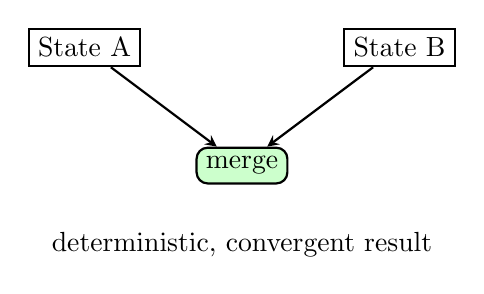
\begin{tikzpicture}[>=stealth, thick]
\node[draw] (s1) at (0,0){State A};
\node[draw] (s2) at (4,0){State B};
\node[draw,rounded corners,fill=green!20] (m) at (2,-1.5){merge};

\draw[->] (s1) -- (m);
\draw[->] (s2) -- (m);

\node at (2,-2.5){deterministic, convergent result};
\end{tikzpicture}
\end{center}
\end{frame}

% ---------- Slide 25 ----------
\begin{frame}{CRDT Convergence — Solutions}
\begin{itemize}
    \item \textbf{Commutative updates} so order does not matter.
    \item \textbf{Associative merge operations} for consistent folding.
    \item \textbf{Idempotent merges} to handle duplicate state.
    \item \textbf{State-based CRDTs} for robust reconciliation.
    \item \textbf{Grow-only or monotonic structures} to avoid conflicts.
\end{itemize}
\end{frame}

% ---------- Slide 26 ----------
\begin{frame}{CRDT — Version Vector Update Algorithm}
\begin{algorithm}[H]
\footnotesize
\caption{Version Vector Update}
\begin{algorithmic}[1]
\State vv[node] $\gets$ vv[node] + 1
\State attach(operation, vv)
\State broadcast(operation)
\State onReceive(op):
\State \hspace{1.5em} vv[op.src] $\gets$ max(vv[op.src], op.vv[op.src])
\State \hspace{1.5em} apply(op)
\end{algorithmic}
\end{algorithm}
\end{frame}

% ----------------------------------------------------------
\section{Failure Models}
% ----------------------------------------------------------

% ---------- Slide 27 ----------
\begin{frame}{Crash-Stop Failures}
\begin{block}{Problem}
Nodes may halt permanently due to hardware faults or power loss. They never recover or rejoin, reducing available replicas and risking loss of majority quorums.
\end{block}

\begin{center}
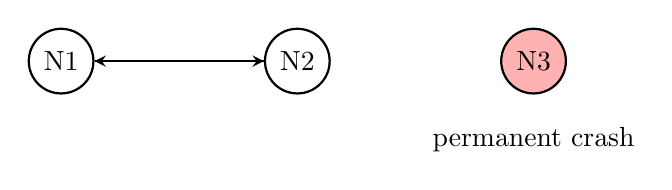
\begin{tikzpicture}[>=stealth, thick]
\node[draw,circle] (n1) at (0,0){N1};
\node[draw,circle] (n2) at (3,0){N2};
\node[draw,circle,fill=red!30] (n3) at (6,0){N3};

\draw[->] (n1) -- (n2);
\draw[->] (n2) -- (n1);

\node at (6,-1){permanent crash};
\end{tikzpicture}
\end{center}
\end{frame}

% ---------- Slide 28 ----------
\begin{frame}{Crash-Stop — Solutions}
\begin{itemize}
    \item \textbf{Majority quorums} to tolerate permanent minority loss.
    \item \textbf{Replicated logs} to keep state despite node loss.
    \item \textbf{Leader re-election} to maintain progress.
    \item \textbf{Durable writes} that survive local crashes.
    \item \textbf{Static membership} for predictable fault tolerance.
\end{itemize}
\end{frame}

% ---------- Slide 29 ----------
\begin{frame}{Crash-Recovery Log Reconstruction}
\begin{algorithm}[H]
\footnotesize
\caption{Crash-Recovery Log Rebuild}
\begin{algorithmic}[1]
\State onStartup():
\State \hspace{1.5em} log $\gets$ loadFromDisk()
\State \hspace{1.5em} lastIndex $\gets$ log.tail
\State \hspace{1.5em} send(hello, peers)
\State \hspace{1.5em} missing $\gets$ fetchEntries(lastIndex, peers)
\State \hspace{1.5em} append(log, missing)
\State \hspace{1.5em} restoreState(log)
\end{algorithmic}
\end{algorithm}
\end{frame}

% ---------- Slide 30 ----------
\begin{frame}{Byzantine Failures}
\begin{block}{Problem}
Nodes may behave arbitrarily: forging messages, equivocating, or selectively dropping updates. This breaks assumptions in non-Byzantine protocols and can mislead peers.
\end{block}

\begin{center}
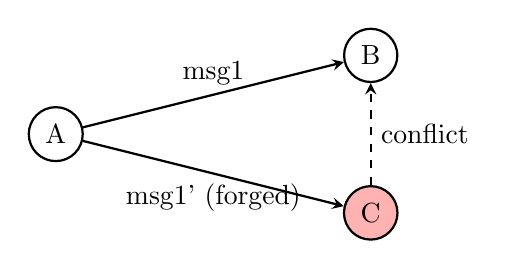
\begin{tikzpicture}[>=stealth, thick]
\node[draw,circle] (a) at (0,0){A};
\node[draw,circle] (b) at (4,1){B};
\node[draw,circle,fill=red!30] (c) at (4,-1){C};

\draw[->] (a) -- (b) node[midway,above]{msg1};
\draw[->] (a) -- (c) node[midway,below]{msg1' (forged)};
\draw[->,dashed] (c) -- (b) node[midway,right]{conflict};
\end{tikzpicture}
\end{center}
\end{frame}

% ==========================================================
% WEEK 2 — MODELS OF DISTRIBUTED COMPUTATION
% CHUNK D — FIXED SLIDES 31–42
% ==========================================================

\section{Distributed Time and Ordering}

% ---------- Slide 31 ----------
\begin{frame}{Lamport Clocks}
\begin{block}{Problem}
Without synchronized clocks, processes cannot agree on the order of events using physical time. Concurrent events make real-time ordering ambiguous.
\end{block}

\begin{center}
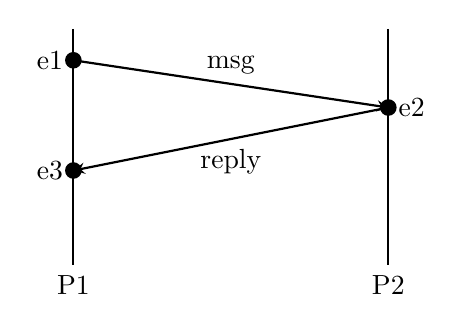
\begin{tikzpicture}[>=stealth, thick, node distance=2cm]

\draw (0,0) -- (0,-3) node[below]{P1};
\draw (4,0) -- (4,-3) node[below]{P2};

\fill (0,-0.4) circle(3pt) node[left]{e1};
\fill (0,-1.8) circle(3pt) node[left]{e3};
\fill (4,-1.0) circle(3pt) node[right]{e2};

\draw[->] (0,-0.4) -- (4,-1.0) node[midway,above]{msg};
\draw[->] (4,-1.0) -- (0,-1.8) node[midway,below]{reply};

\end{tikzpicture}
\end{center}
\end{frame}

% ---------- Slide 32 ----------
\begin{frame}{Lamport Clocks — Solutions}
\begin{itemize}
    \item \textbf{Monotonic counters} incremented on each event.
    \item \textbf{Piggyback timestamps} on every message.
    \item \textbf{Max-merge rule} to update local clocks.
    \item \textbf{Defines happens-before} without physical time.
    \item \textbf{Total order} via tie-breaking with process ID.
\end{itemize}
\end{frame}

% ---------- Slide 33 ----------
\begin{frame}{Lamport Clock Update Algorithm}
\begin{algorithm}[H]
\footnotesize
\caption{Lamport Timestamp Update}
\begin{algorithmic}[1]

\State onLocalEvent():
\State \hspace{1.5em} clock \(\gets\) clock + 1

\State onSend(msg):
\State \hspace{1.5em} clock \(\gets\) clock + 1
\State \hspace{1.5em} msg.ts \(\gets\) clock
\State \hspace{1.5em} send(msg)

\State onReceive(msg):
\State \hspace{1.5em} clock \(\gets\) \(\max(clock,\ msg.ts) + 1\)

\end{algorithmic}
\end{algorithm}
\end{frame}

% ----------------------------------------------------------
\section{Happens-Before}
% ----------------------------------------------------------

% ---------- Slide 34 ----------
\begin{frame}{Happens-Before Relation}
\begin{block}{Problem}
Determining causality between events is difficult without a global timeline. Concurrent events appear unordered in real time.
\end{block}

\begin{center}
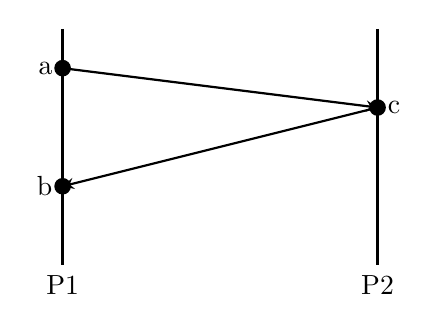
\begin{tikzpicture}[>=stealth, thick]

\draw (0,0) -- (0,-3) node[below]{P1};
\draw (4,0) -- (4,-3) node[below]{P2};

\fill (0,-0.5) circle(3pt) node[left]{a};
\fill (0,-2.0) circle(3pt) node[left]{b};
\fill (4,-1.0) circle(3pt) node[right]{c};

\draw[->] (0,-0.5) -- (4,-1.0);
\draw[->] (4,-1.0) -- (0,-2.0);

\end{tikzpicture}
\end{center}
\end{frame}

% ---------- Slide 35 ----------
\begin{frame}{Happens-Before — Solutions}
\begin{itemize}
    \item \textbf{Lamport timestamps} encode causal precedence.
    \item \textbf{HB defines concurrency} when neither event dominates.
    \item \textbf{Prevents reordering errors} in replicated logs.
    \item \textbf{Supports deterministic replay}.
    \item \textbf{Enables causal consistency} across replicas.
\end{itemize}
\end{frame}

% ----------------------------------------------------------
\section{Vector Clocks}
% ----------------------------------------------------------

% ---------- Slide 36 ----------
\begin{frame}{Vector Clocks}
\begin{block}{Problem}
Lamport clocks cannot distinguish true concurrency from causality. Systems require richer metadata to track causality accurately.
\end{block}

\begin{center}
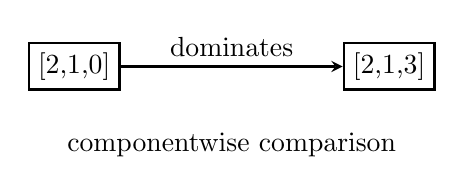
\begin{tikzpicture}[>=stealth, thick]
\node[draw] (v1) at (1,0) {{[2,1,0]}};
\node[draw] (v2) at (5,0) {{[2,1,3]}};

\draw[->] (v1) -- (v2) node[midway,above]{dominates};

\node at (3,-1){componentwise comparison};
\end{tikzpicture}
\end{center}
\end{frame}

% ---------- Slide 37 ----------
\begin{frame}{Vector Clocks — Solutions}
\begin{itemize}
    \item \textbf{Track causality} per process dimension.
    \item \textbf{Detect concurrency} using vector comparison rules.
    \item \textbf{Support multi-writer replication}.
    \item \textbf{Drive conflict resolution} in CRDTs.
    \item \textbf{Minimal metadata} for consistent ordering.
\end{itemize}
\end{frame}

% ---------- Slide 38 ----------
\begin{frame}{Vector Clock Update Algorithm}
\begin{algorithm}[H]
\footnotesize
\caption{Vector Clock Update}
\begin{algorithmic}[1]

\State onLocalEvent():
\State \hspace{1.5em} VC[i] \(\gets\) VC[i] + 1

\State onSend(op):
\State \hspace{1.5em} VC[i] \(\gets\) VC[i] + 1
\State \hspace{1.5em} op.VC \(\gets\) VC

\State onReceive(op):
\State \hspace{1.5em} \For{each process j}
    \State \hspace{3em} VC[j] \(\gets\) \(\max(VC[j],\ op.VC[j])\)
\EndFor
\State \hspace{1.5em} VC[i] \(\gets\) VC[i] + 1

\end{algorithmic}
\end{algorithm}
\end{frame}

% ----------------------------------------------------------
\section{Gossip Dissemination}
% ----------------------------------------------------------

% ---------- Slide 39 ----------
\begin{frame}{Gossip Dissemination}
\begin{block}{Problem}
Broadcasting updates reliably in large clusters is expensive. Loss or delays slow convergence if updates aren't propagated probabilistically.
\end{block}

\begin{center}
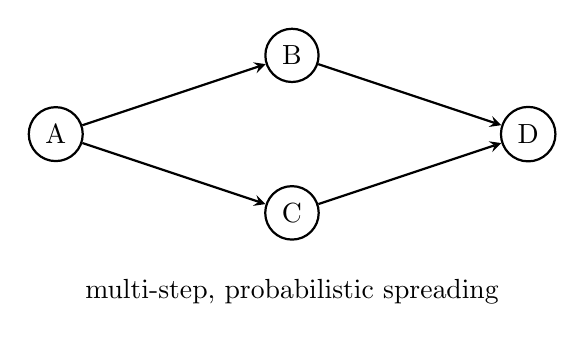
\begin{tikzpicture}[>=stealth, thick]
\node[draw,circle] (a) at (0,0){A};
\node[draw,circle] (b) at (3,1){B};
\node[draw,circle] (c) at (3,-1){C};
\node[draw,circle] (d) at (6,0){D};

\draw[->] (a) -- (b);
\draw[->] (a) -- (c);
\draw[->] (b) -- (d);
\draw[->] (c) -- (d);

\node at (3,-2){multi-step, probabilistic spreading};
\end{tikzpicture}
\end{center}
\end{frame}

% ---------- Slide 40 ----------
\begin{frame}{Gossip — Solutions}
\begin{itemize}
    \item \textbf{Random peer selection} to avoid bottlenecks.
    \item \textbf{Push-pull exchange} to accelerate convergence.
    \item \textbf{Periodic rounds} for steady dissemination.
    \item \textbf{Rumor-mongering} to limit message load.
    \item \textbf{Epidemic-style propagation} for scalability.
\end{itemize}
\end{frame}

% ---------- Slide 41 ----------
\begin{frame}{Gossip Round Algorithm}
\begin{algorithm}[H]
\footnotesize
\caption{Push-Pull Gossip}
\begin{algorithmic}[1]
\While{true}
    \State wait(roundInterval)
    \State peer \(\gets\) pickRandom()
    \State send(localState,\ peer)
    \State remote \(\gets\) receive(peer)
    \State localState \(\gets\) merge(localState,\ remote)
\EndWhile
\end{algorithmic}
\end{algorithm}
\end{frame}

% ----------------------------------------------------------
\section{Consistent Hashing}
% ----------------------------------------------------------

% ---------- Slide 42 ----------
\begin{frame}{Consistent Hashing}
\begin{block}{Problem}
When nodes join or leave, naive sharding causes large-scale data movement. Systems need key distribution that minimizes redistribution.
\end{block}

\begin{center}
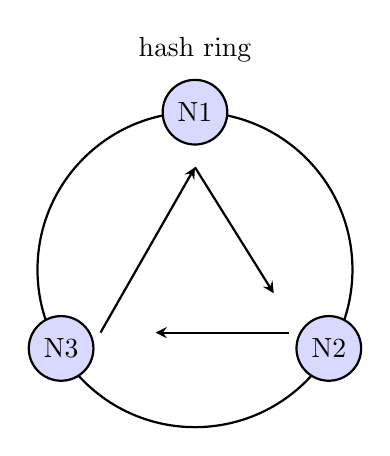
\begin{tikzpicture}[>=stealth, thick]
\draw[thick] (0,0) circle (2cm);

\node at (0,2.8){hash ring};

\node[draw,circle,fill=blue!15] (n1) at (0,2){N1};
\node[draw,circle,fill=blue!15] (n2) at (1.7,-1){N2};
\node[draw,circle,fill=blue!15] (n3) at (-1.7,-1){N3};

\draw[->] (0,1.3) -- (1,-0.3);
\draw[->] (1.2,-0.8) -- (-0.5,-0.8);
\draw[->] (-1.2,-0.8) -- (0,1.3);

\end{tikzpicture}
\end{center}
\end{frame}

